
\documentclass[12pt,a4paper]{article} 

\usepackage{float,times,graphicx,mathtools}
\usepackage{amsmath}
\usepackage{amsfonts}
\usepackage{amssymb}
\usepackage{latexsym}
\usepackage{epsfig}
\usepackage{graphicx}
\usepackage{caption}
\usepackage{subcaption}
\usepackage{color}
\usepackage{pdfpages}
\usepackage{natbib}
\usepackage[space]{grffile}
\usepackage{wrapfig}
\usepackage{subcaption}
\usepackage{url}
\usepackage{bbm}
\usepackage{tikzsymbols}

\DeclareMathOperator{\logit}{logit}
\DeclareMathOperator{\tr}{tr}
\bibpunct[, ]{(}{)}{;}{a}{,}{,}
\graphicspath{{../}}  
\addtolength{\oddsidemargin}{-1in}
	\addtolength{\evensidemargin}{-1in}
	\addtolength{\textwidth}{1.75in}
	\addtolength{\topmargin}{-1.3in}
	\addtolength{\textheight}{2in}
\date{\vspace{-5ex}}
\begin{document}


\begin{itemize}
\item Fitted to only females
\item Estimated population counts are very similar across models with different priors on the LogQuad parameters
\item raw UNPD census counts exhibits age heaping problems, which are reflected in the estimated migration proportions $g_x$
\item Used WPP 1960 population estimates as baseline, from age 0 to 85+
\item Estimated $_5q_0$ are mostly lower than the IGME estimates, except when the weighted mean prior is used
\item Estimated $_{45}q_{15}$ lower than WPP estimates most of the time
\item DHS raw mortality rates don't seem to be under-represented according to the estimated LogQuad models
\item Cannot converge for joint sex projection, unless the open age group is reduced to 80+ (possibly because WPP 1960 estimates for 85+ were 0?)
\item Tried fitting the model to both males and females, however estimates for male mortality rates are much lower than the IGME estimates again
\begin{itemize}
\item[--] Tried using male population counts and fit it to the female model, estimates remain unchanged, so probably not a coding error, but will double check again
\end{itemize}
\end{itemize}

\newpage
\begin{figure}[H]
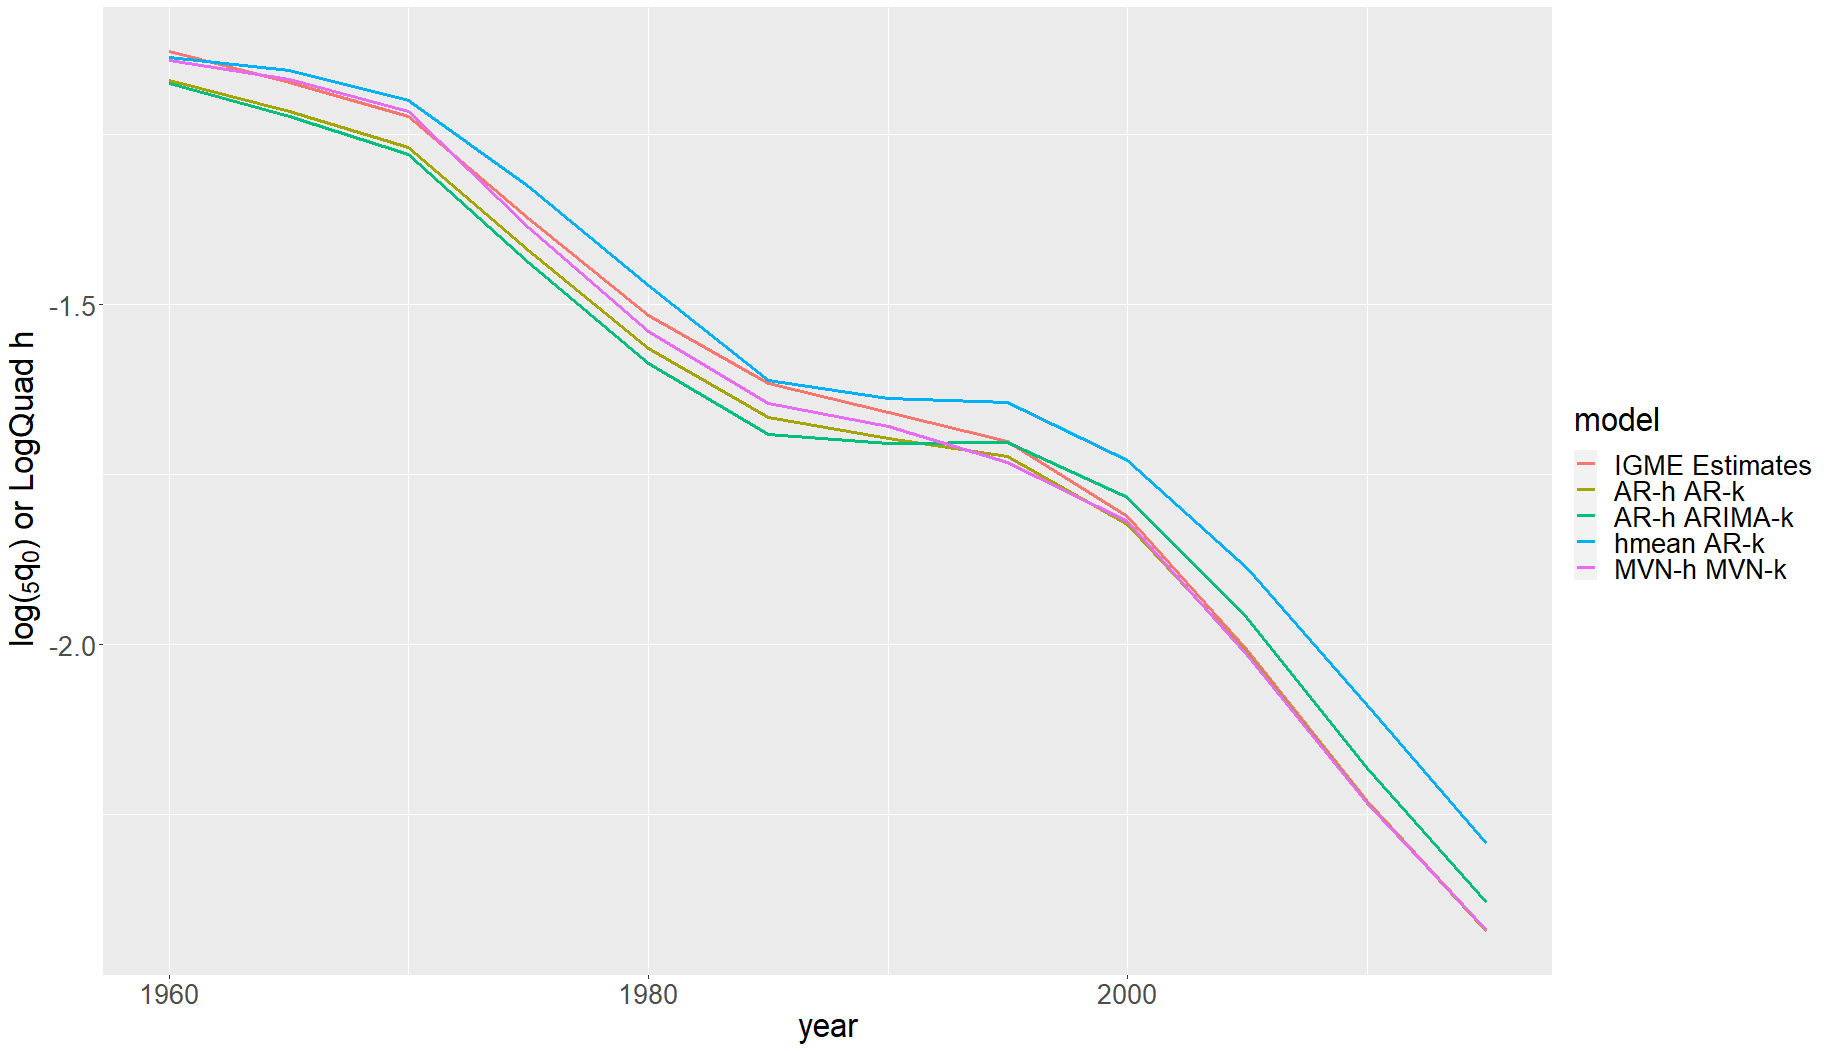
\includegraphics[width = \linewidth]{Burkina Faso/6/h.png}
\caption{Estimated $h$}
\end{figure}
\begin{figure}[H]
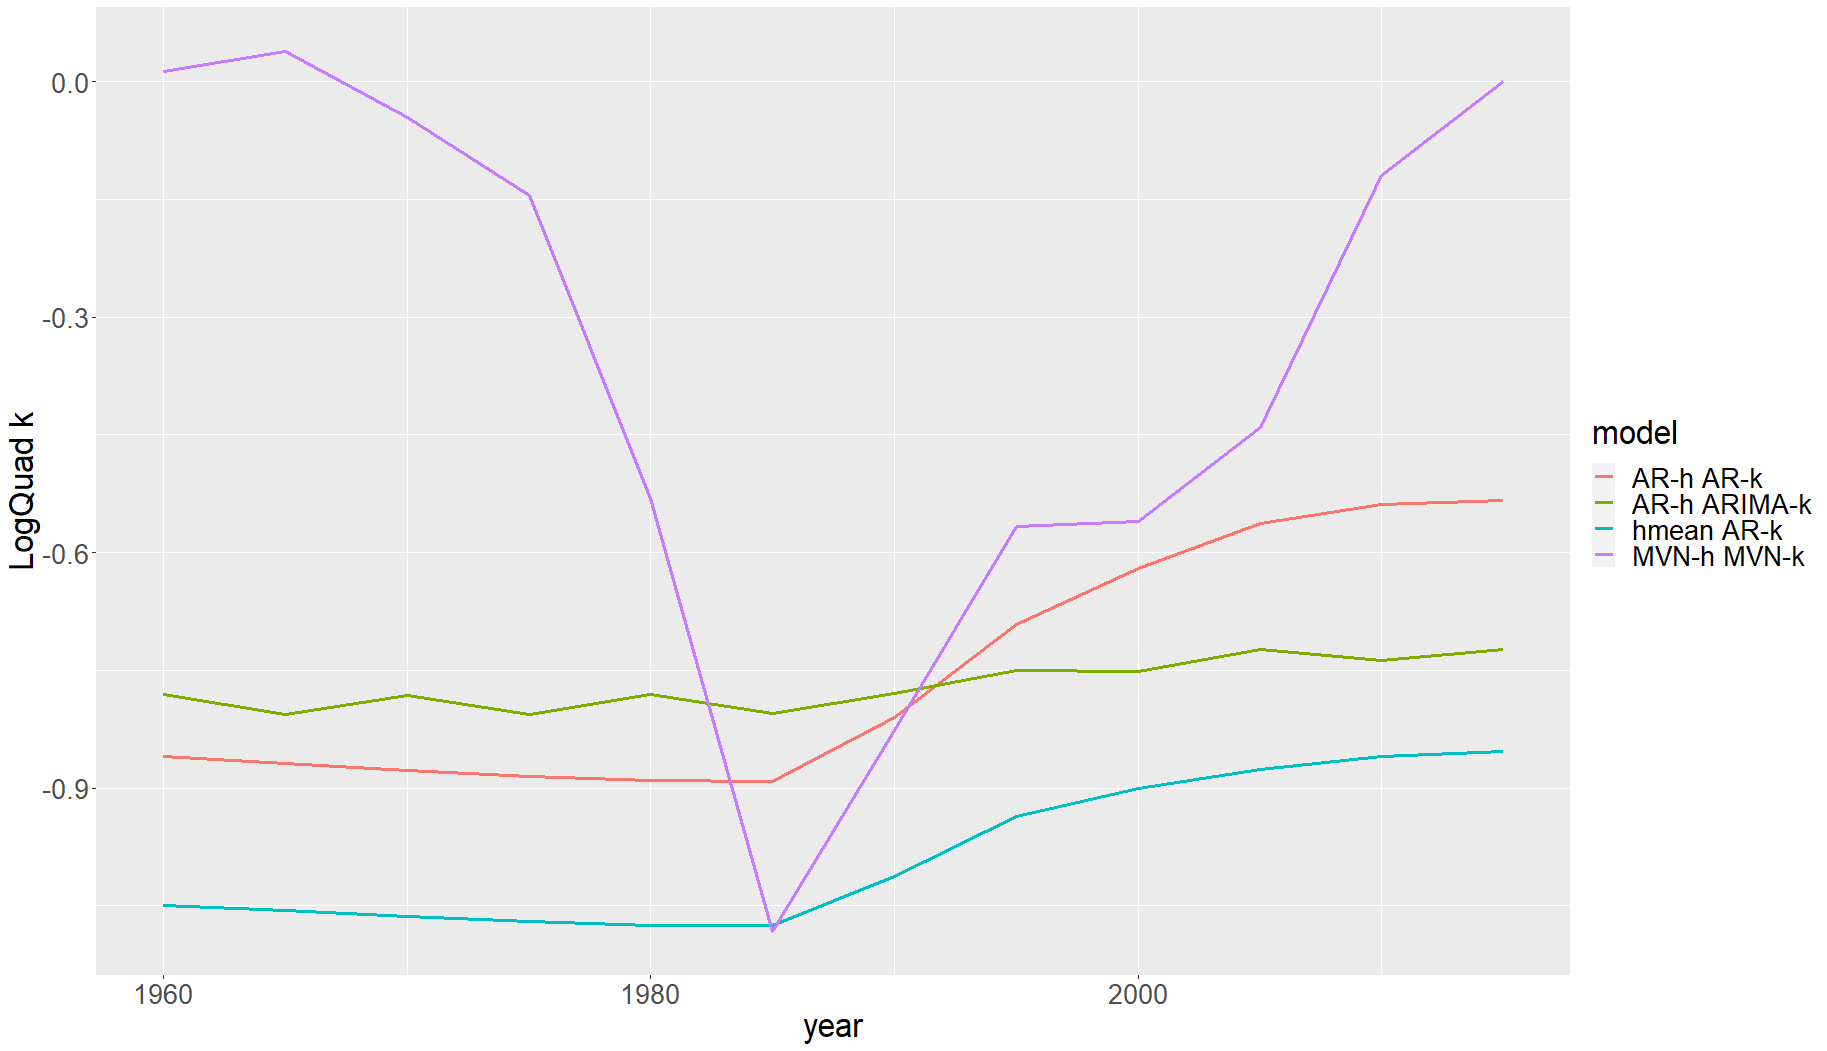
\includegraphics[width = \linewidth]{Burkina Faso/6/k.png}
\caption{Estimated $k$}
\end{figure}

\newpage
\begin{figure}[H]
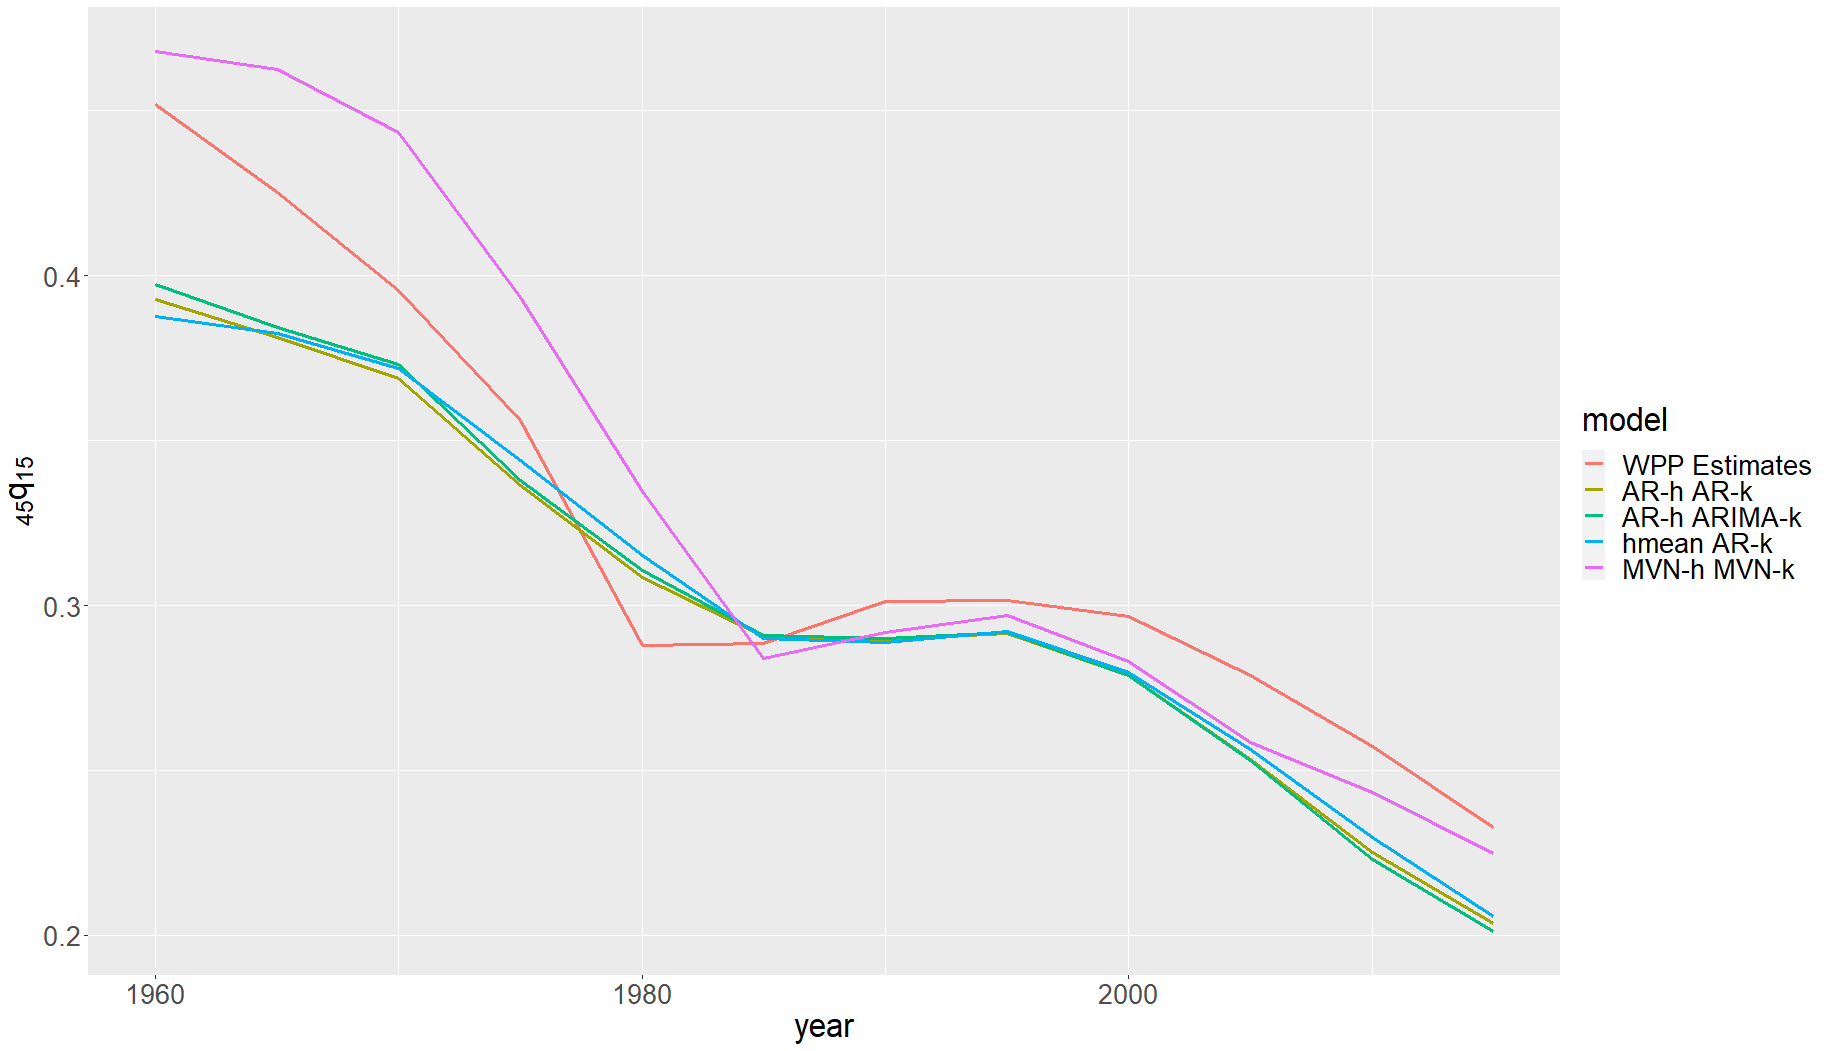
\includegraphics[width = \linewidth]{Burkina Faso/6/q4515.png}
\caption{Estimated $_{45}q_{15}$}
\end{figure}
\newpage
\begin{figure}[H]
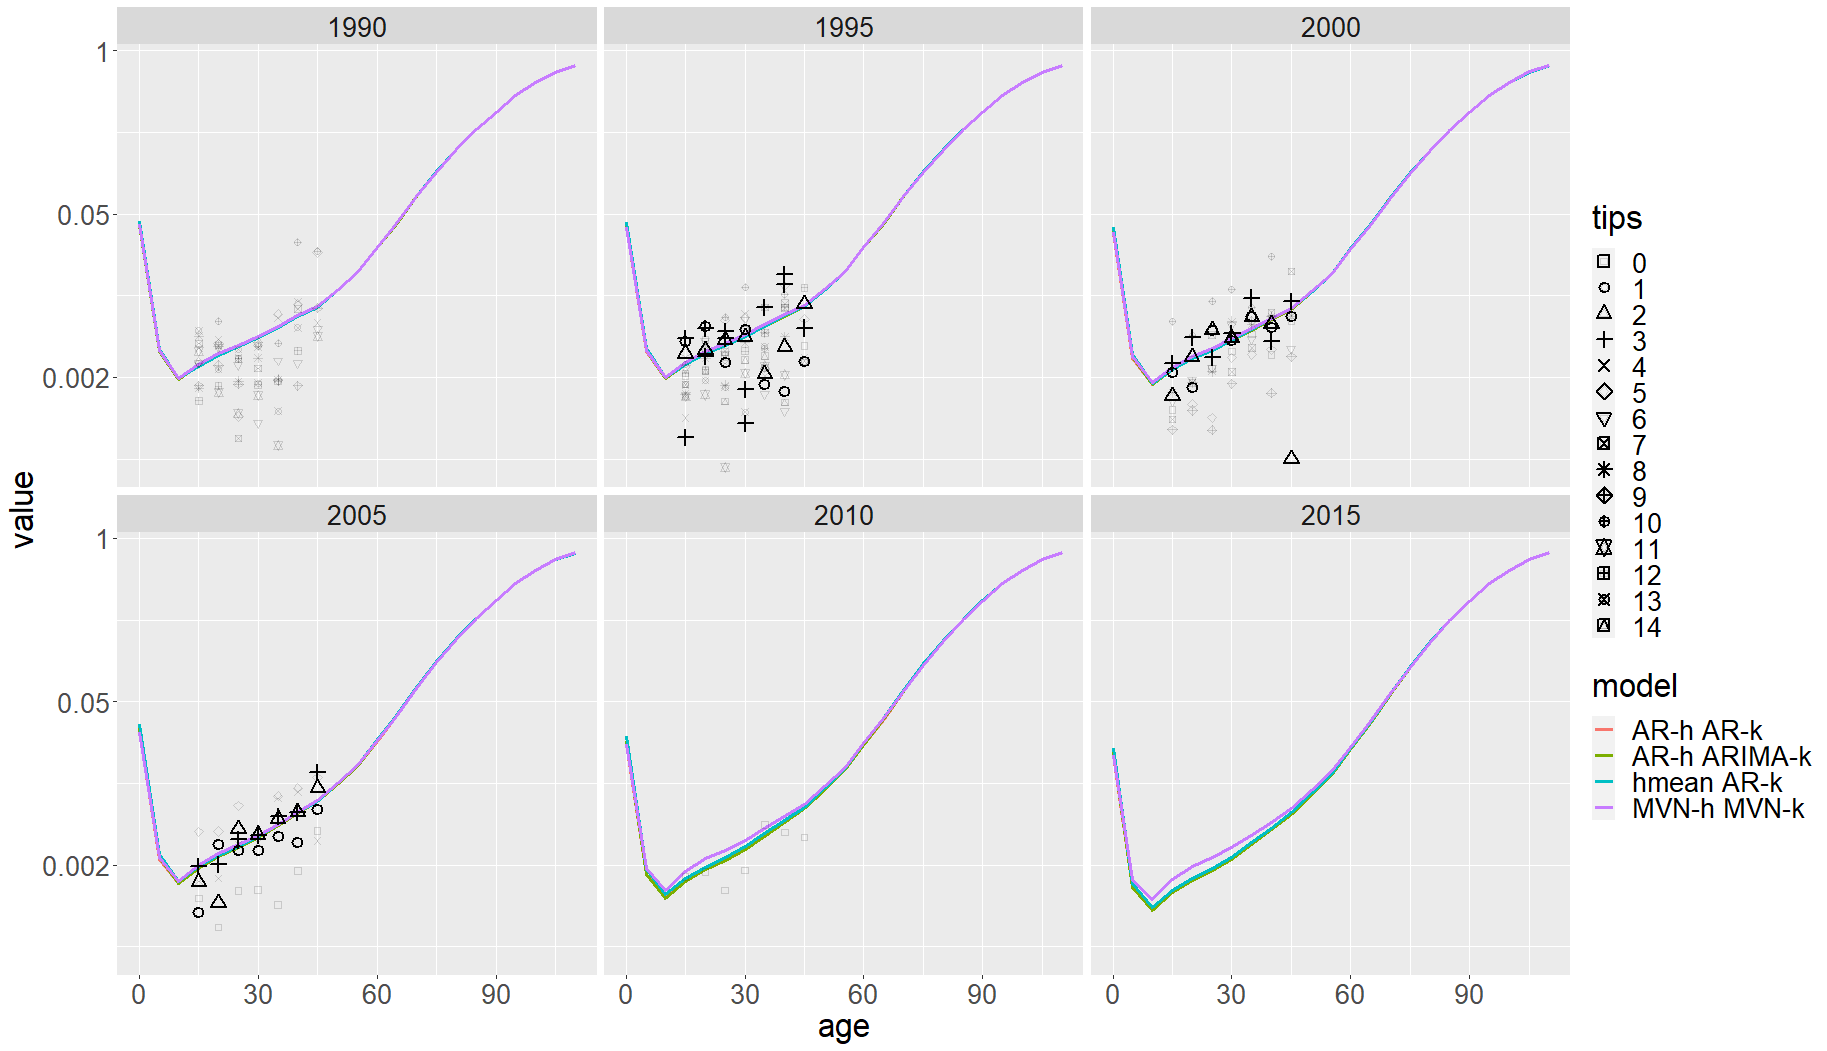
\includegraphics[width = \linewidth]{Burkina Faso/6/period mx.png}
\caption{Estimated period mortality rates}
\end{figure}
\begin{figure}[H]
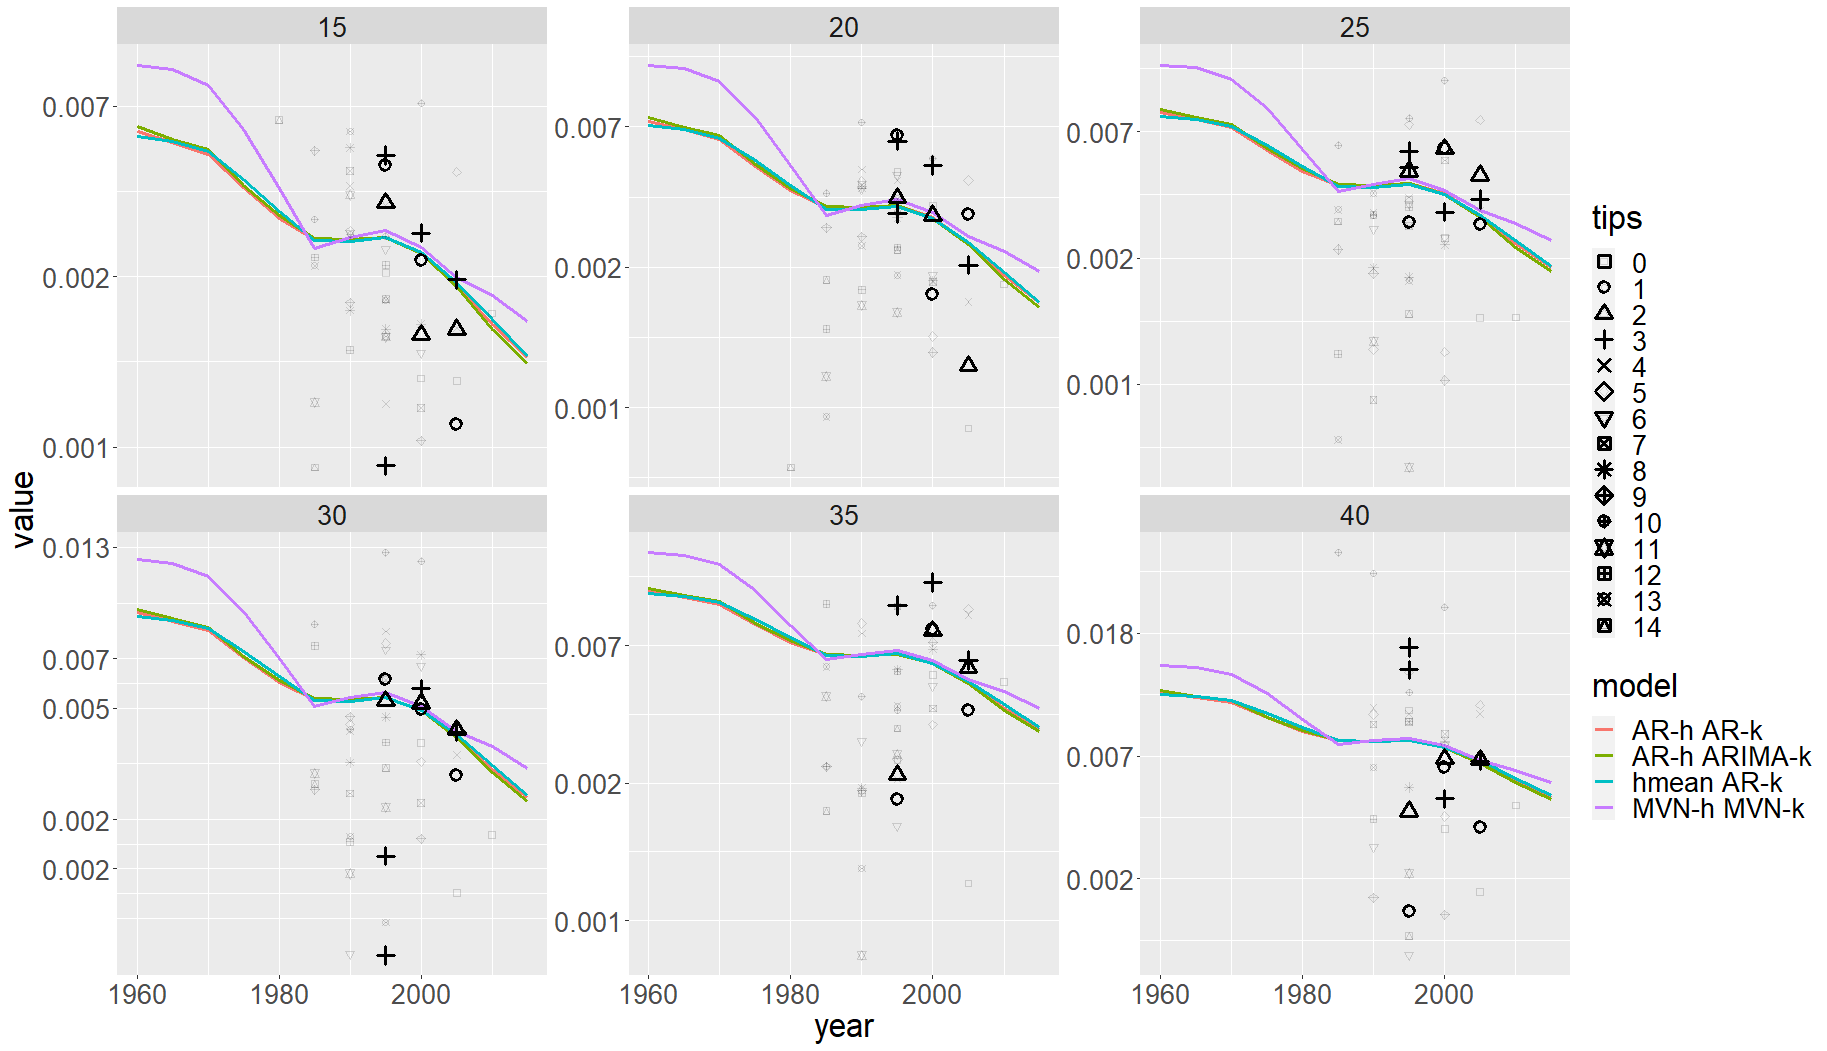
\includegraphics[width = \linewidth]{Burkina Faso/6/age mx.png}
\caption{Estimated period mortality rates}
\end{figure}

\newpage
\begin{figure}[H]
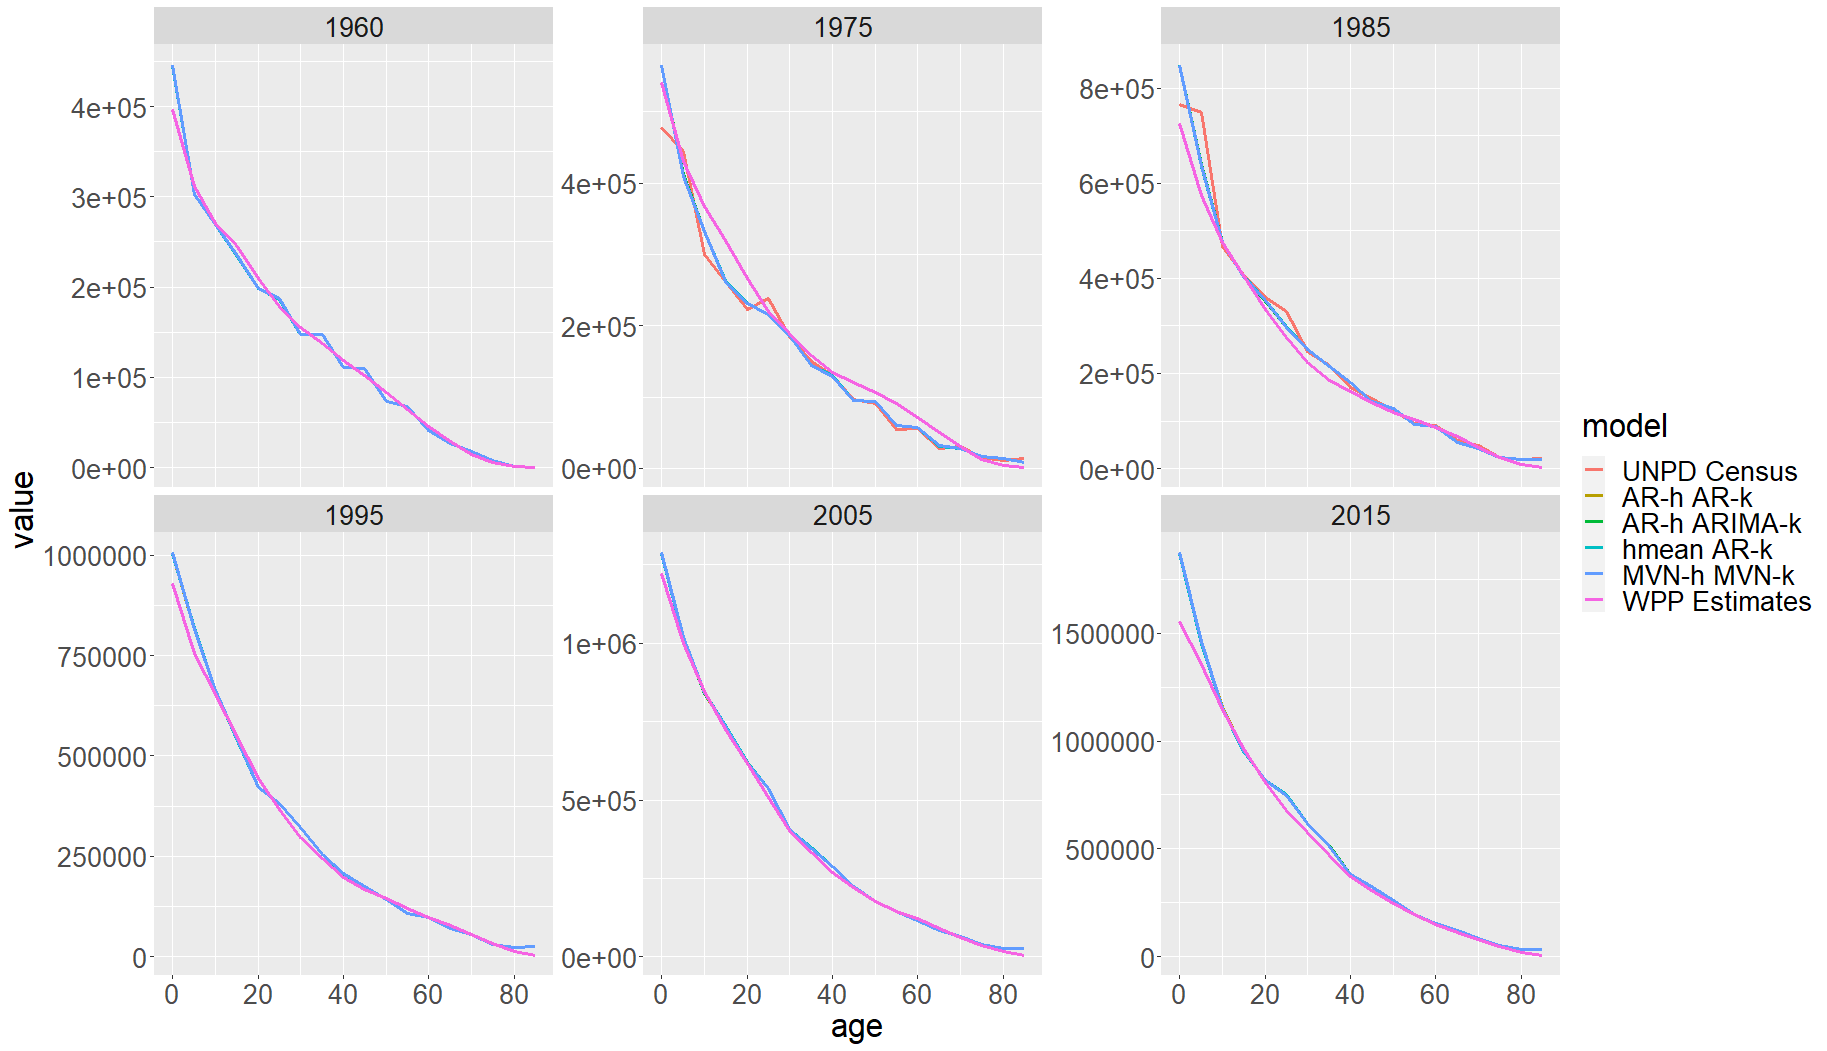
\includegraphics[width = \linewidth]{Burkina Faso/6/period pop.png} 	
\caption{Estimated population counts in different years}
\end{figure}
\begin{figure}[H]
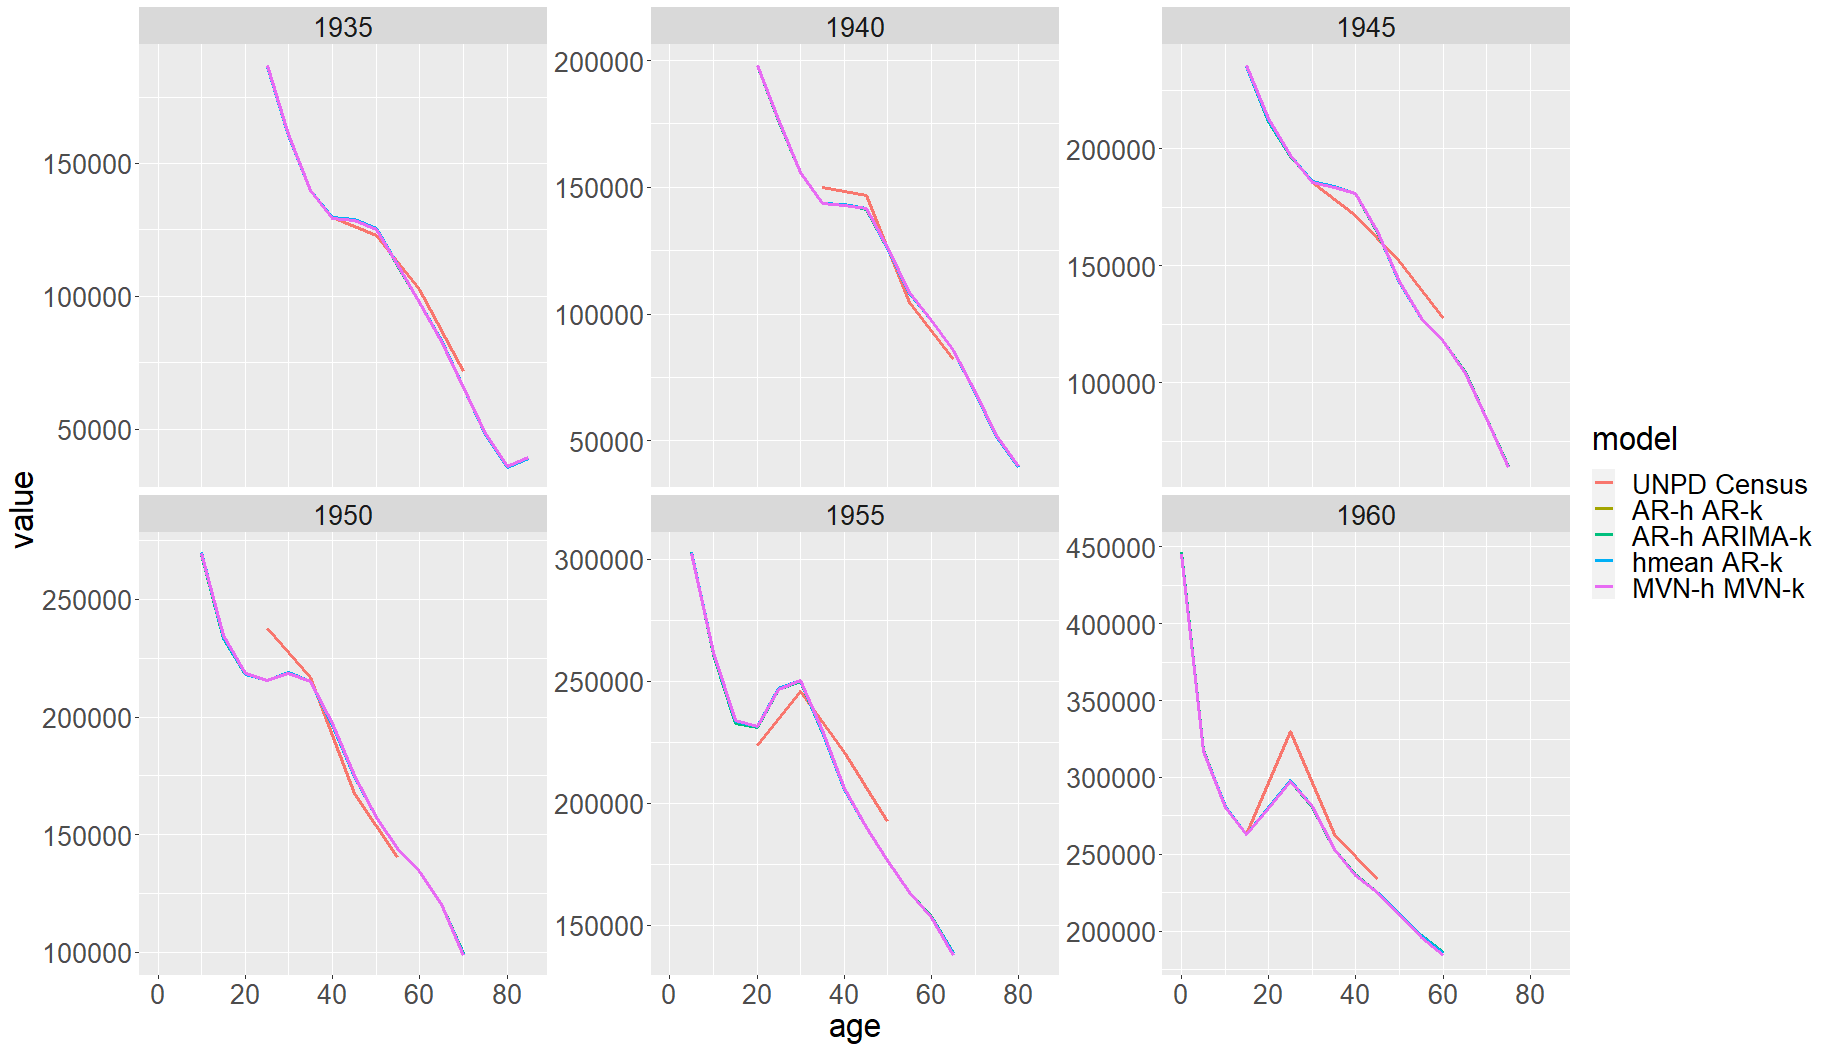
\includegraphics[width = \linewidth]{Burkina Faso/6/cohort pop.png}
\caption{Estimated population counts for different cohorts}
\end{figure}

\newpage
\begin{figure}[H]
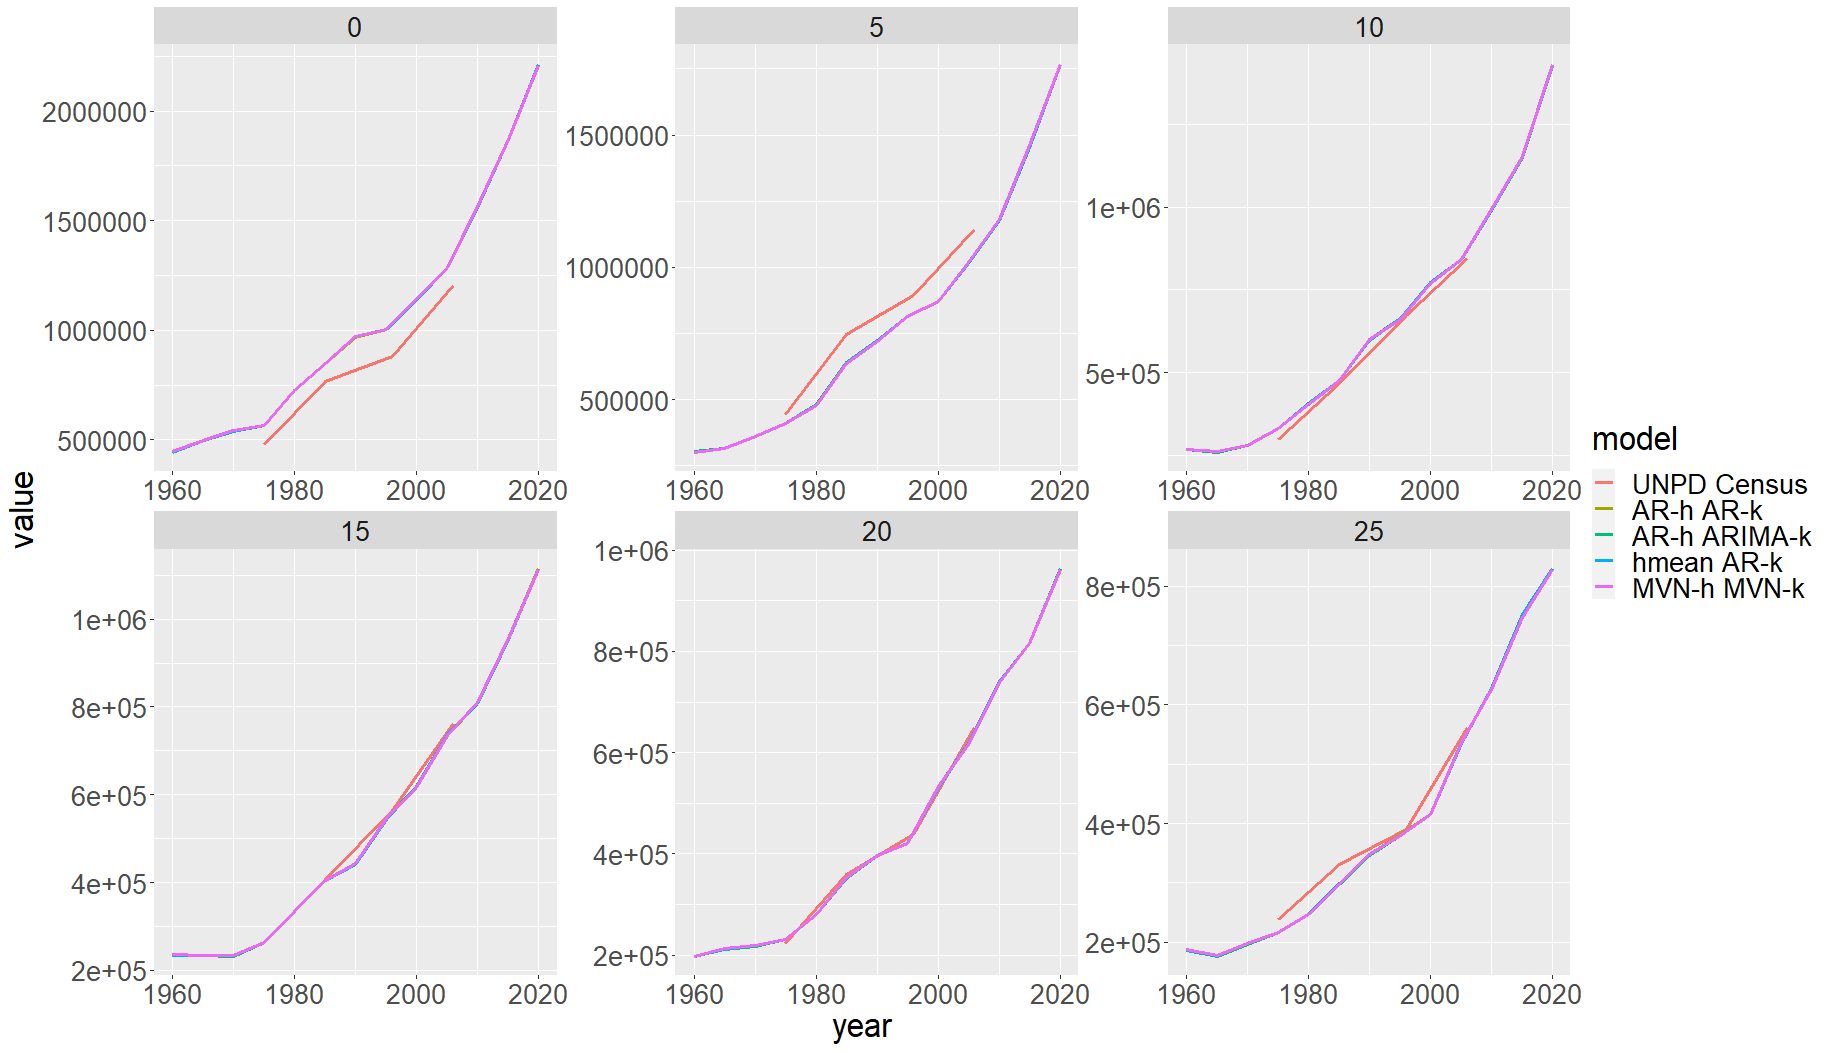
\includegraphics[width = \linewidth]{Burkina Faso/6/age pop.png} 	
\caption{Estimated population counts at different ages}
\end{figure}
\begin{figure}[H]
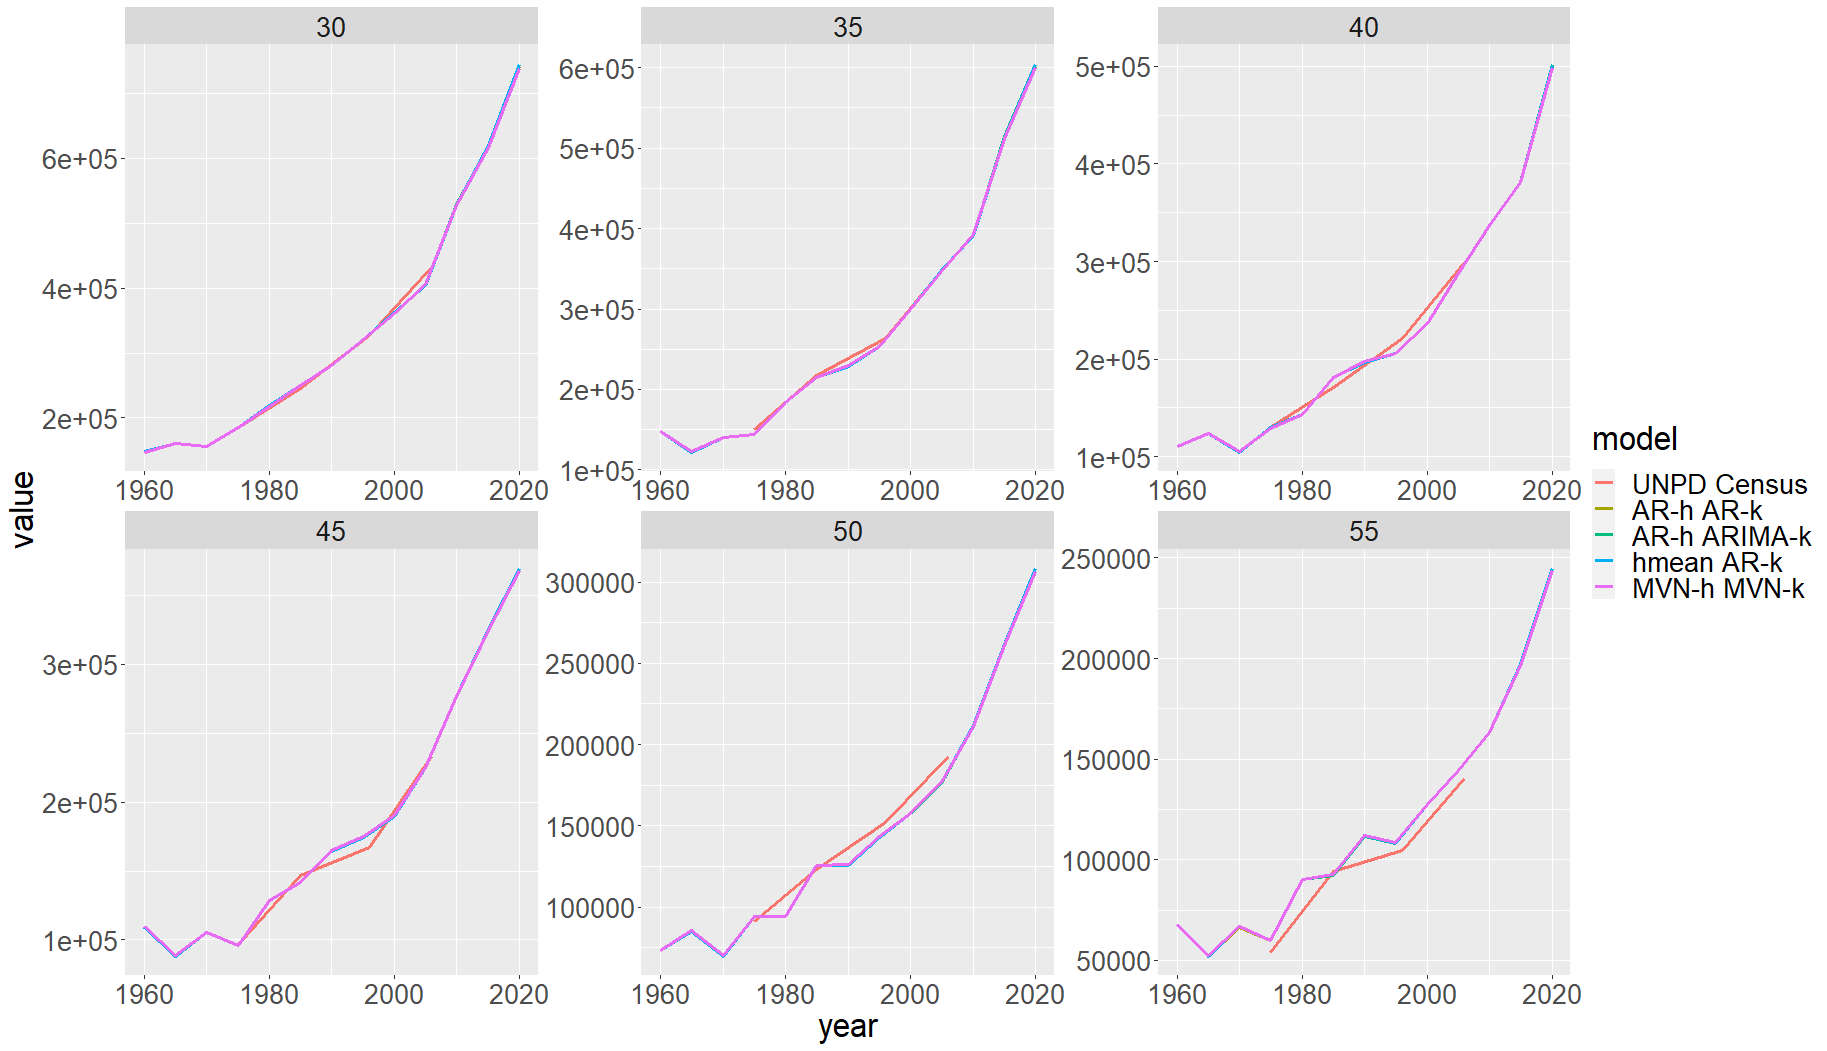
\includegraphics[width = \linewidth]{Burkina Faso/6/age pop 2.png}
\caption{Estimated population counts at different ages}
\end{figure}

\newpage
\begin{figure}[H]
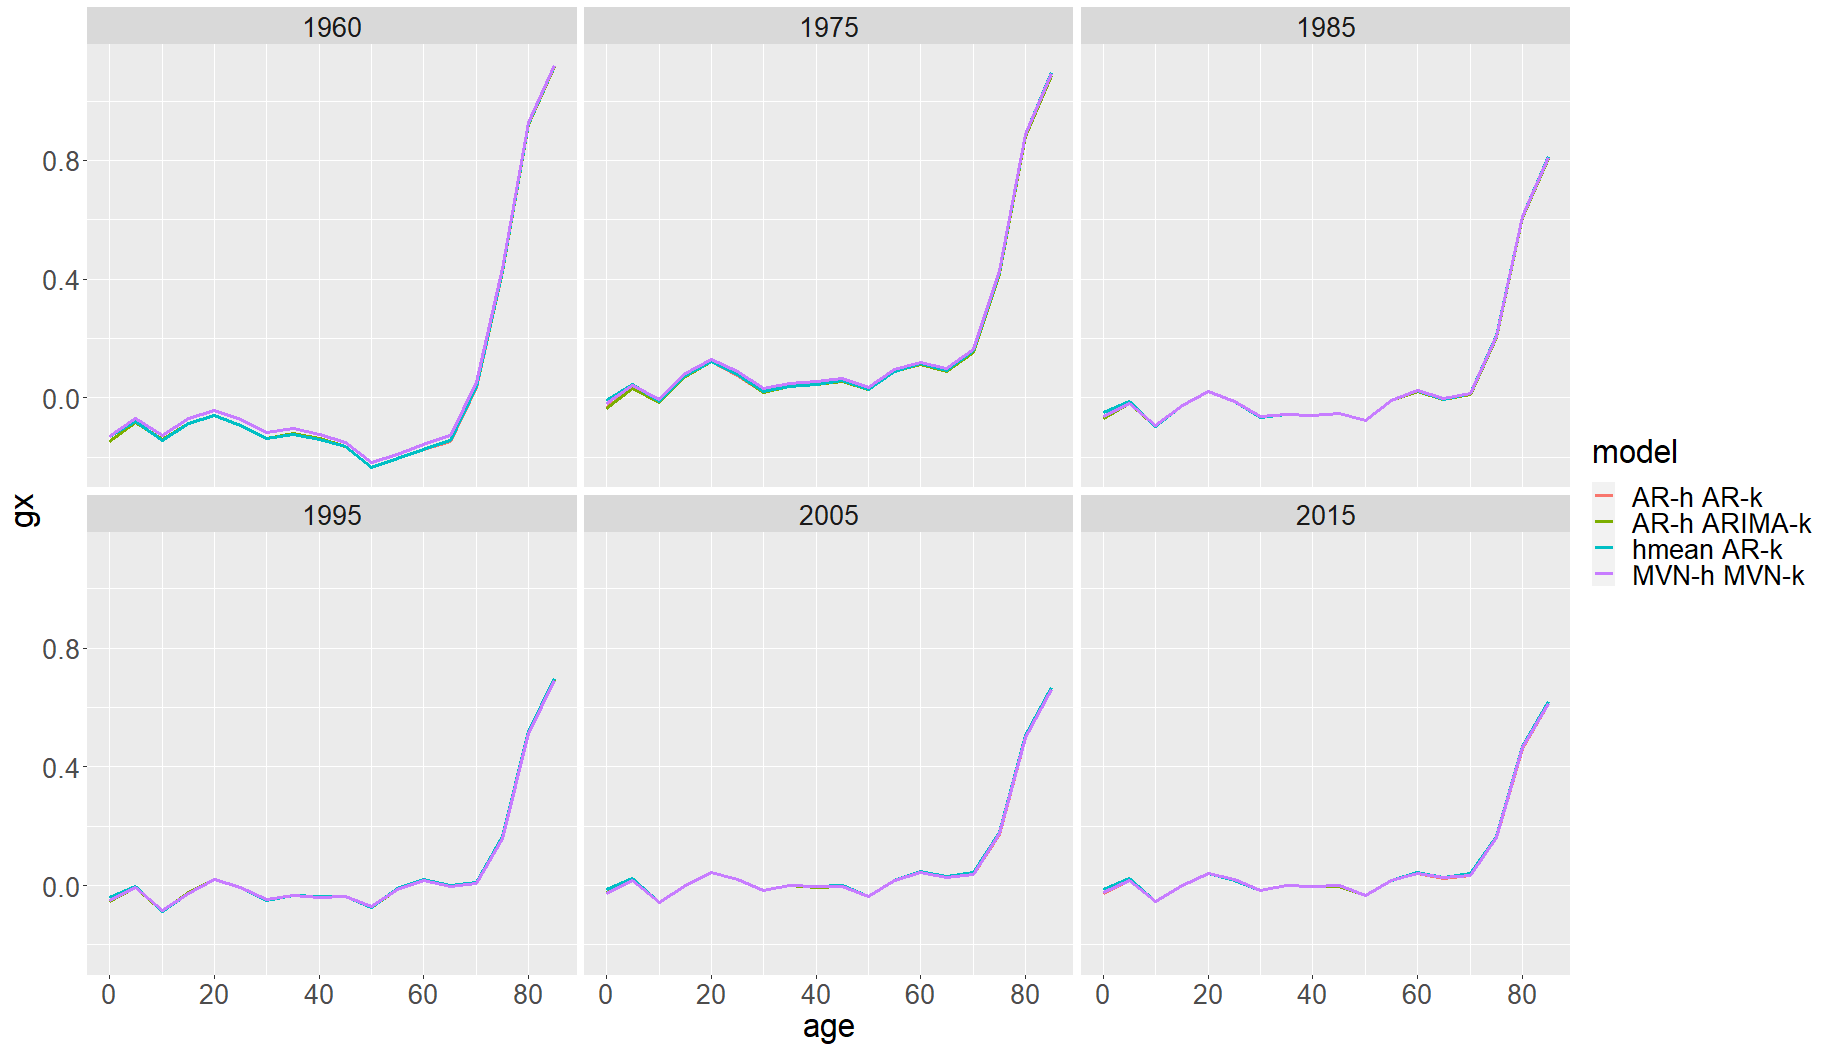
\includegraphics[width = \linewidth]{Burkina Faso/6/period mig.png} 	
\caption{Estimated migration proportions}
\end{figure}
\begin{figure}[H]
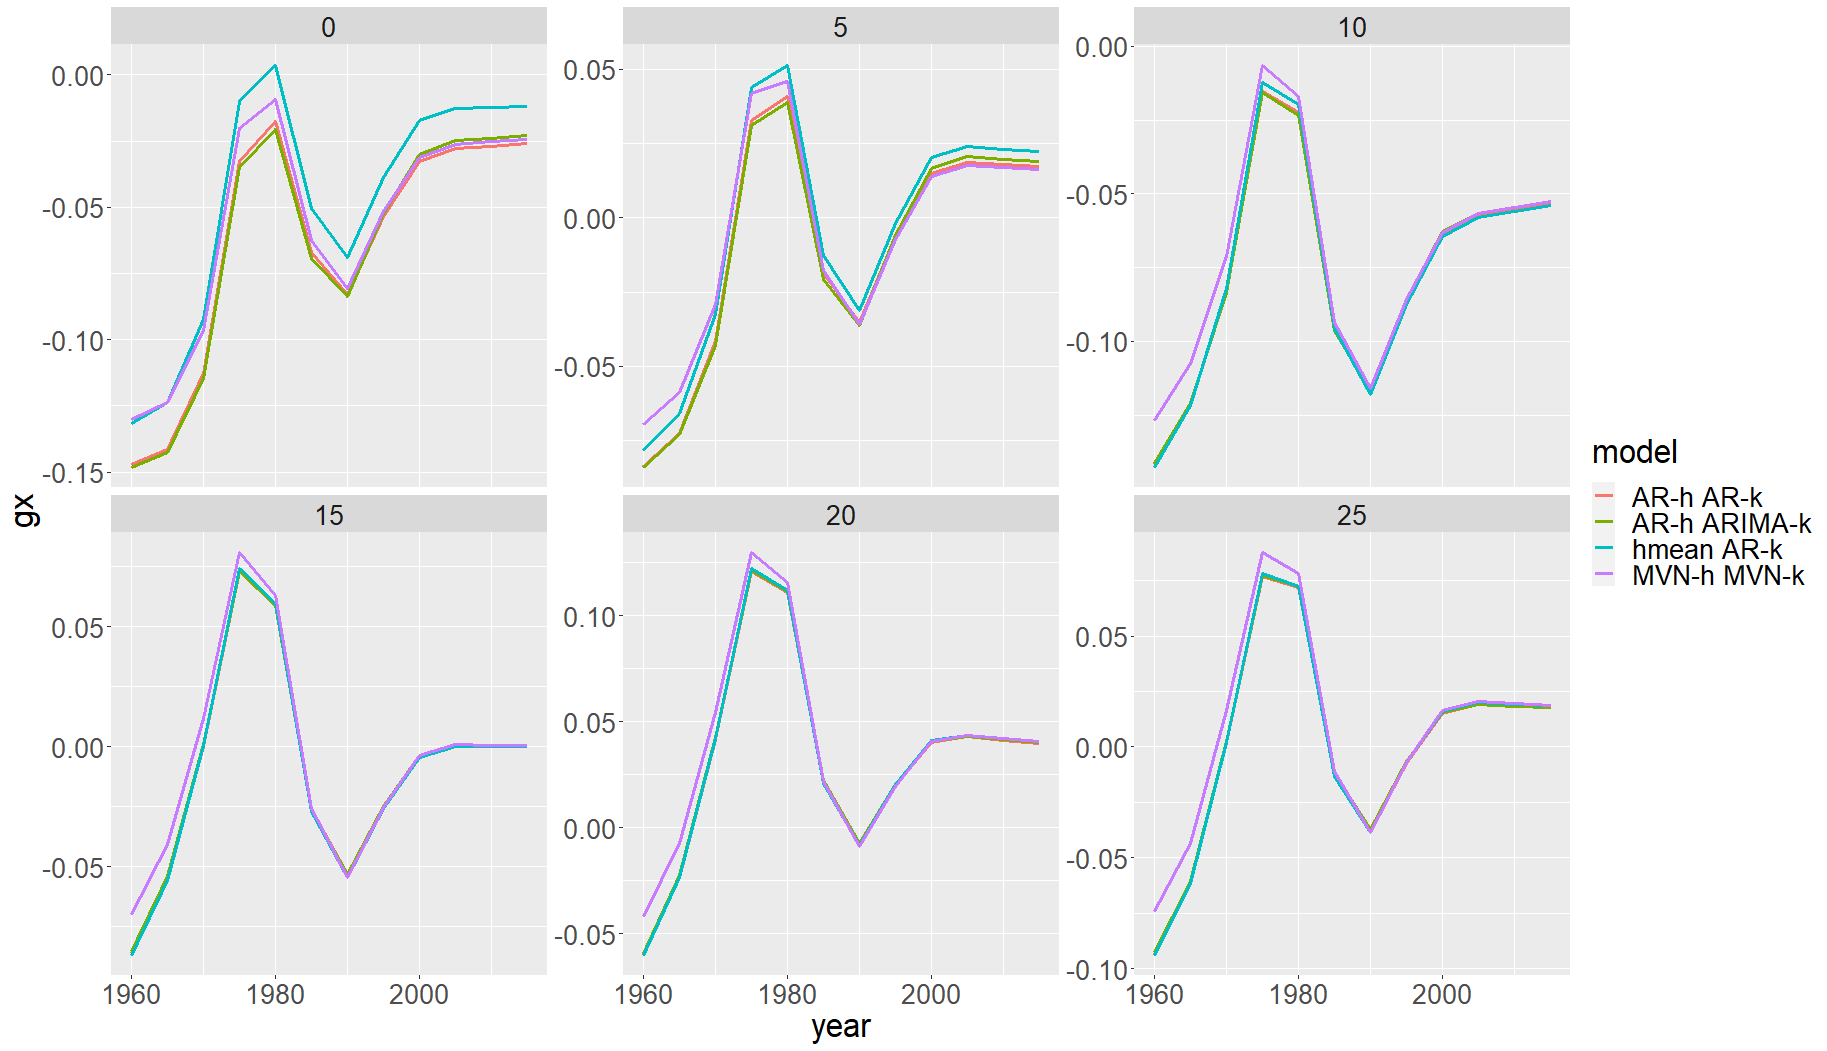
\includegraphics[width = \linewidth]{Burkina Faso/6/age mig.png}
\caption{Estimated migration proportions}
\end{figure}
\begin{figure}[H]
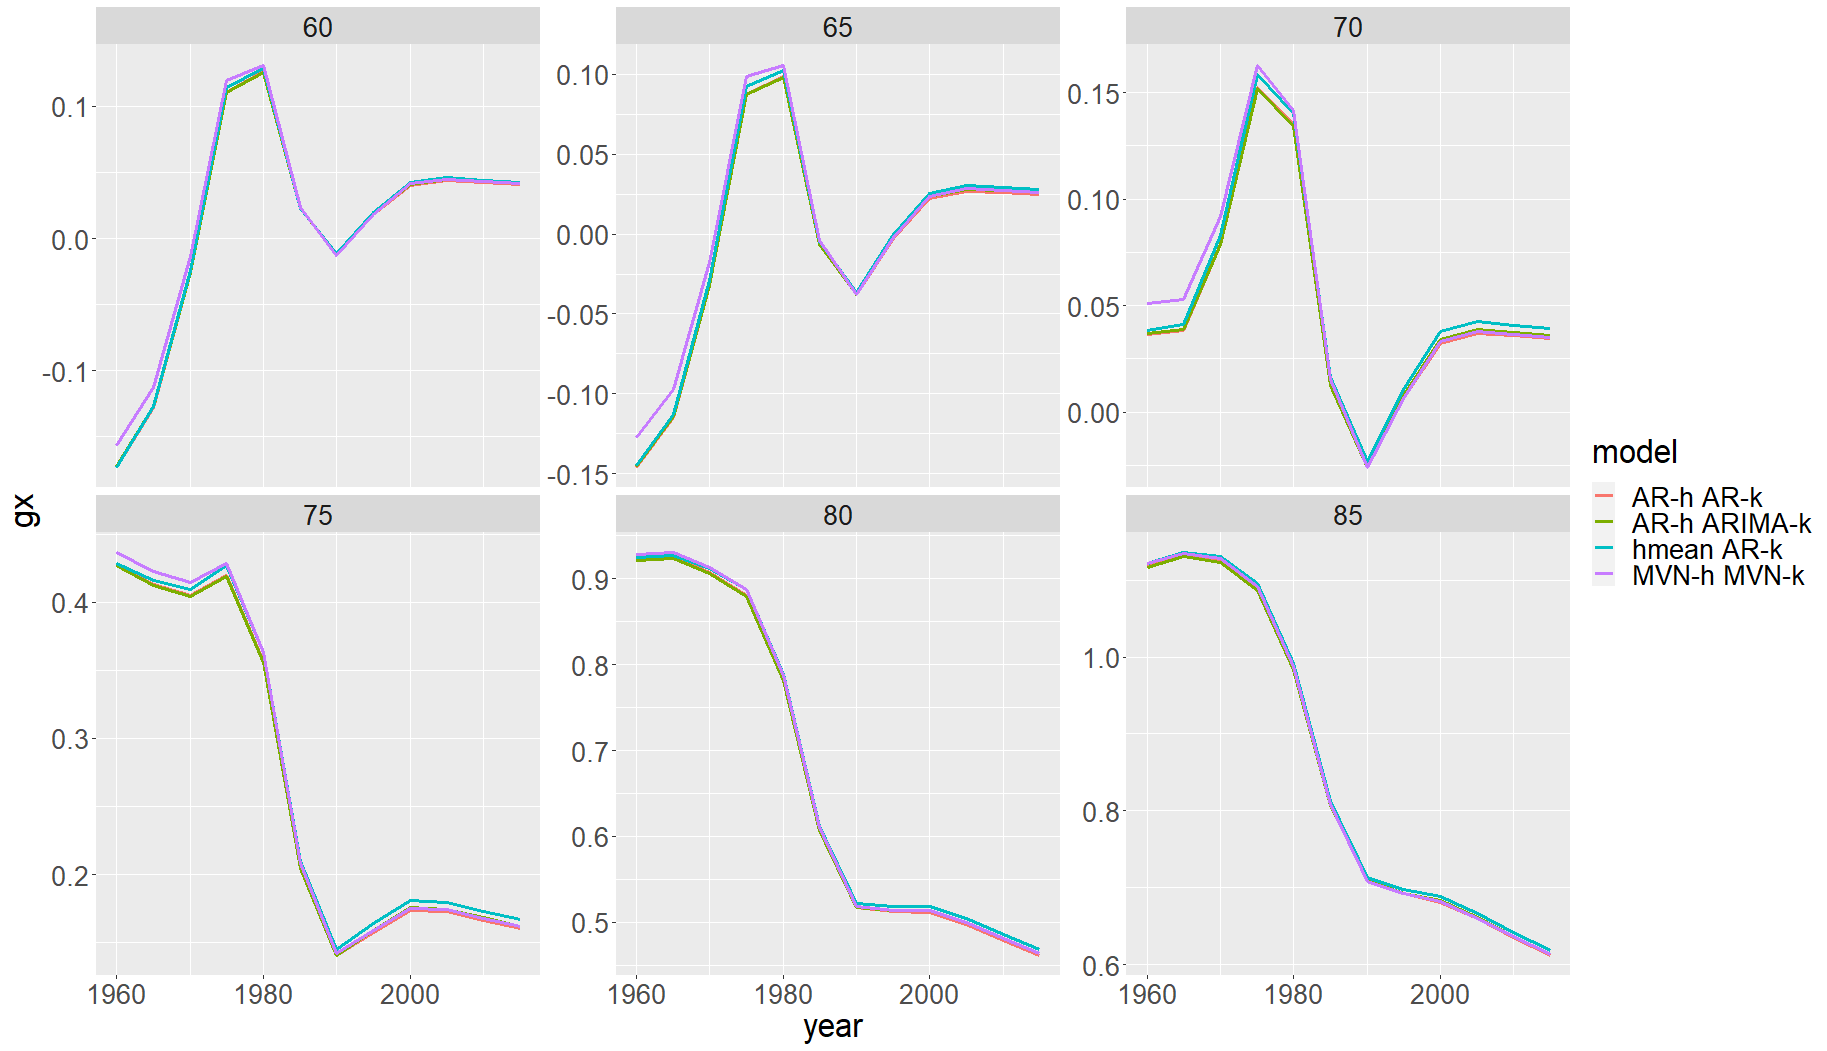
\includegraphics[width = \linewidth]{Burkina Faso/6/age mig 2.png}
\caption{Estimated migration proportions}
\end{figure}

\newpage
\begin{figure}[H]
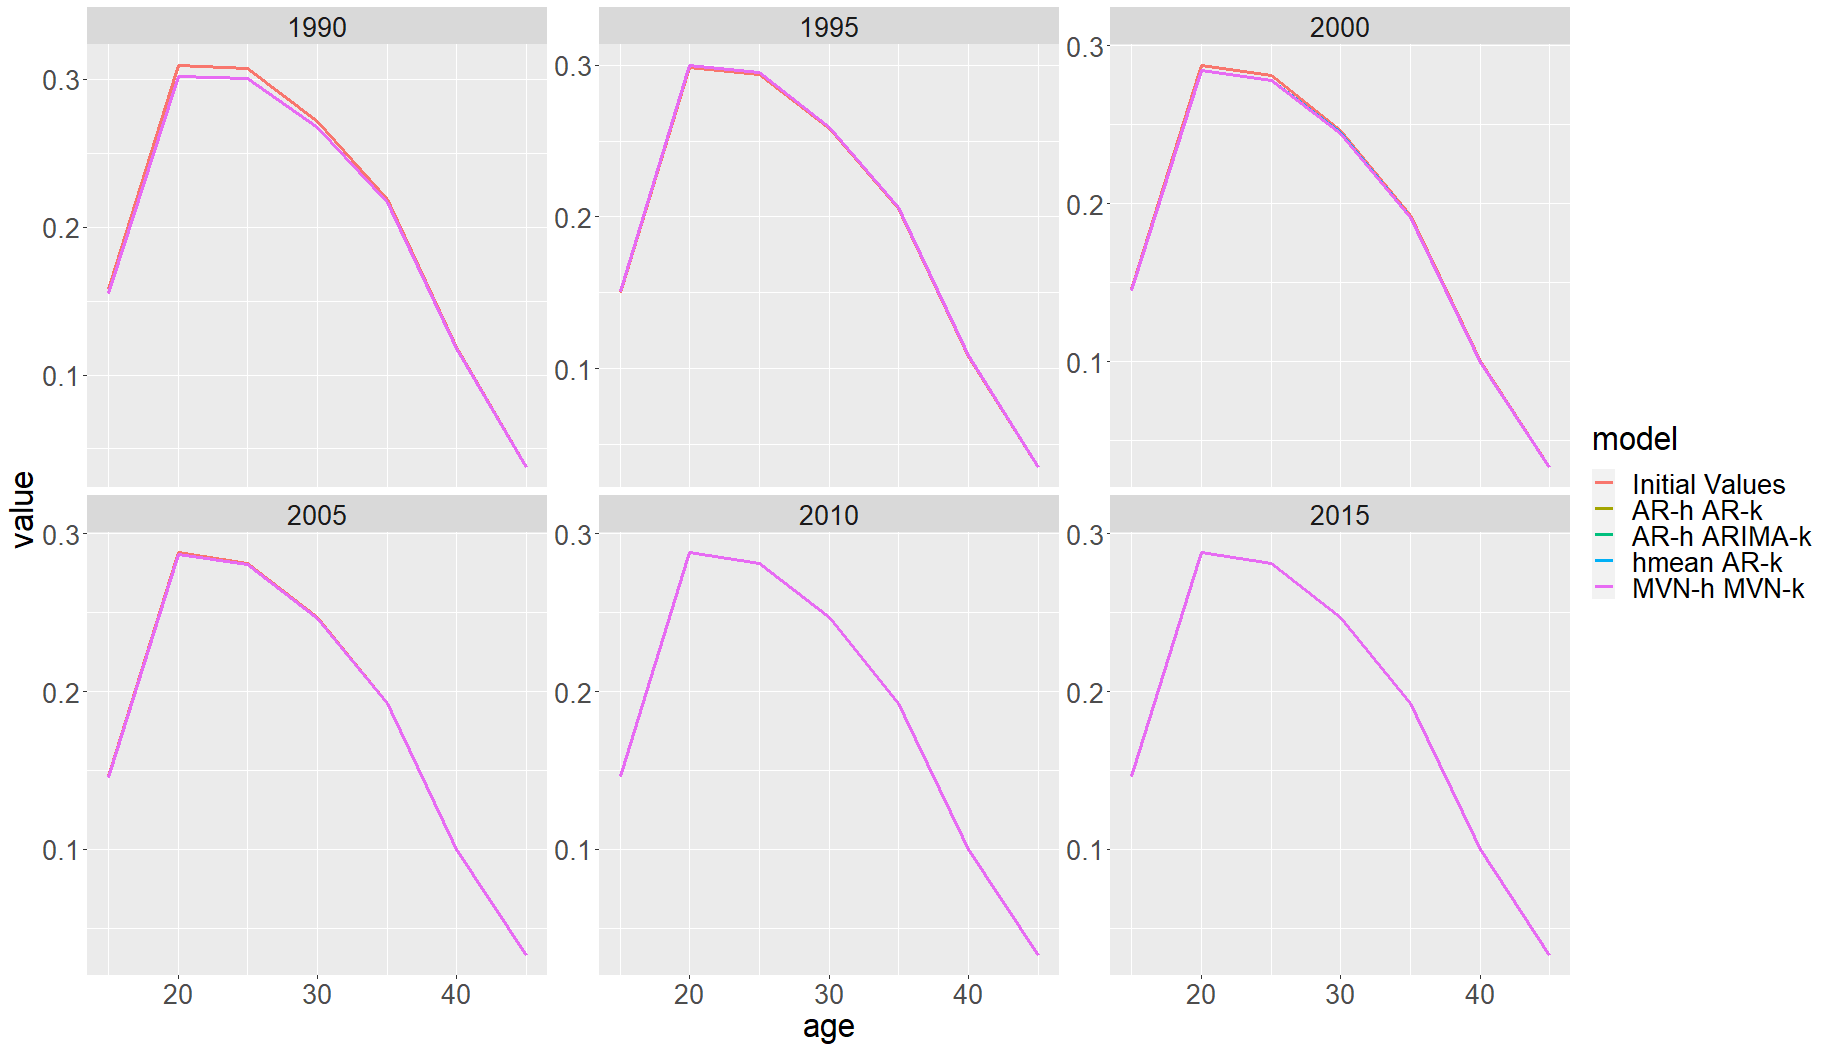
\includegraphics[width = \linewidth]{Burkina Faso/6/period fx.png}
\caption{Estimated fertility}
\end{figure}
\begin{figure}[H]
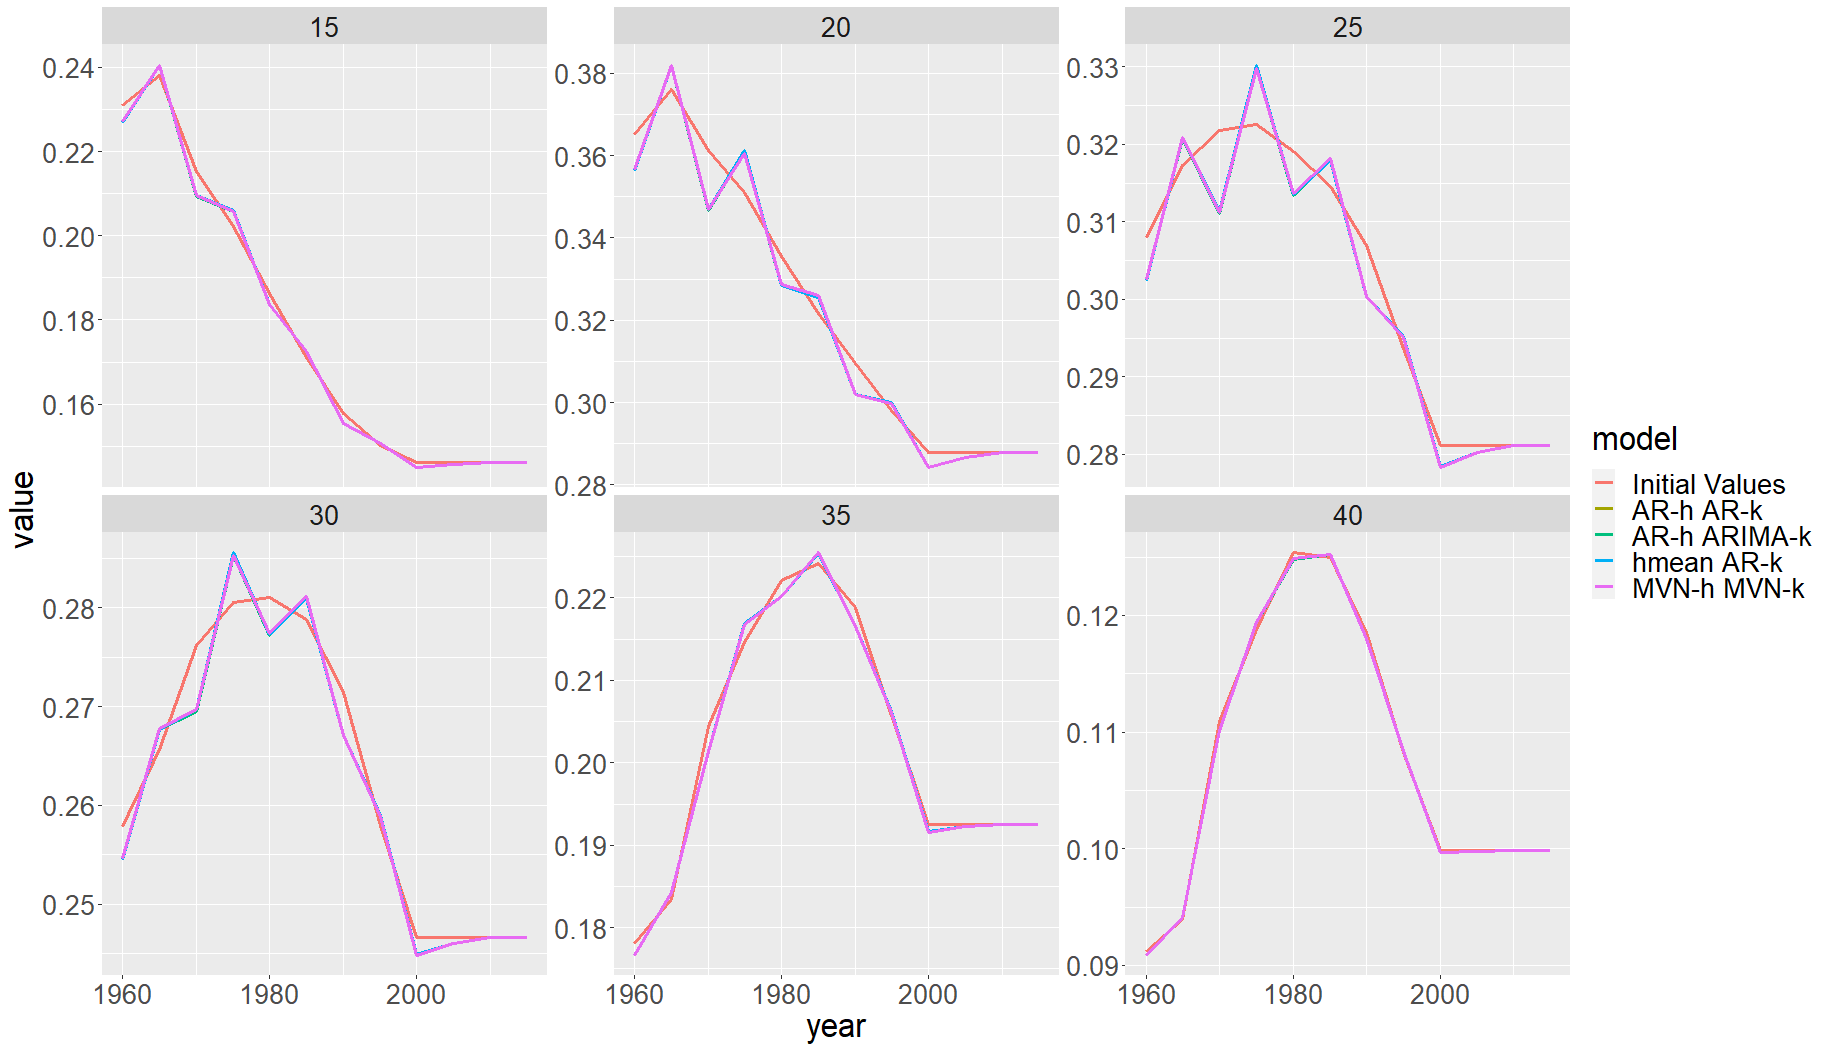
\includegraphics[width = \linewidth]{Burkina Faso/6/age fx.png}
\caption{Estimated fertility}
\end{figure}
\end{document} 